\documentclass[11pt,letterpaper,reqno]{amsart}

%% Solutions to Daron Acemoglu, Introduction to Modern Economic Growth (Princeton, 2009).
%% This document contains the solutions only: the exercise statements are not reproduced,
%% and each exercise is identified by its number in the book.
%% Self-contained: the preamble below is acemoglusol.sty inlined verbatim, so that the
%% document compiles with pdflatex alone.

\makeatletter
\usepackage{amsmath}
\usepackage{amssymb}
\usepackage{amsthm}
\usepackage{mathtools}
\usepackage[margin=1in]{geometry}
\usepackage{enumitem}
\usepackage{booktabs}
\usepackage{setspace}
\usepackage[expansion=false]{microtype}  % expansion off: it can make pdfTeX misplace text
\usepackage{xcolor}
\usepackage{graphicx}
\usepackage{fancyvrb}
\usepackage{bm}

\definecolor{NavyBlue}{RGB}{0,51,153}
\definecolor{RuleGrey}{RGB}{120,120,120}

\usepackage[colorlinks=true,linkcolor=NavyBlue,urlcolor=NavyBlue,
                citecolor=NavyBlue,linktoc=all]{hyperref}

%% ---------------------------------------------------------------------------
%% Layout
%% ---------------------------------------------------------------------------
\onehalfspacing
\allowdisplaybreaks[2]
\setlength{\parindent}{0pt}
\setlength{\parskip}{0.6ex plus 0.2ex minus 0.1ex}
\setlength{\emergencystretch}{2em}
\setlist{nosep,topsep=0.5ex}
\raggedbottom

%% ---------------------------------------------------------------------------
%% Notation.  Acemoglu writes time arguments in parentheses, time derivatives
%% with a dot, and steady-state values with a star; the macros follow him.
%% ---------------------------------------------------------------------------
\newcommand{\R}{\mathbb{R}}
\newcommand{\N}{\mathbb{N}}
\newcommand{\wh}[1]{\widehat{#1}}
\newcommand{\wt}[1]{\widetilde{#1}}
\newcommand{\ol}[1]{\overline{#1}}
\newcommand{\bs}{\boldsymbol}
\newcommand{\dd}{\,\mathrm{d}}
\newcommand{\dt}[1]{\dot{#1}}
\newcommand{\ie}{i.e.\ }
\newcommand{\eg}{e.g.\ }
\DeclareMathOperator{\sgn}{sgn}
\DeclareMathOperator{\rank}{rank}
\DeclareMathOperator*{\argmin}{arg\,min}
\DeclareMathOperator*{\argmax}{arg\,max}

%% ---------------------------------------------------------------------------
%% Exercise environment
%%
%%   \begin{aex}{2.4}{Short title}  ... \solution ... \end{aex}
%%
%% The statement is set in italics, the solution upright.  A short title may be
%% empty: \begin{aex}{2.4}{}.
%% ---------------------------------------------------------------------------
\newcommand{\as@head}[3]{%
  \par\addvspace{1.6ex}\penalty-200\relax
  \phantomsection
  % The bookmark carries the kind and the number only: the short titles contain
  % mathematics, which hyperref cannot turn into a PDF string.
  \addcontentsline{toc}{subsection}{#1 #2\texorpdfstring{\ifx\relax#3\relax\else\quad #3\fi}{}}%
  {\color{RuleGrey}\hrule height 0.4pt}%
  \nobreak\vspace{0.8ex}\nobreak
  \noindent{\bfseries #1 #2}%
  \ifx\relax#3\relax\else\quad{\bfseries\itshape #3}\fi
  \par\nobreak\vspace{0.4ex}\nobreak
  \as@beginstatement
}

% The statement of the exercise is set in italics, in a group that \solution closes.
% The public document carries no statements (tools/build_main.py strips them), and
% redefines this to \ignorespaces so that no group is opened and none is left open.
\newcommand{\as@beginstatement}{\begingroup\itshape\ignorespaces}

\newenvironment{aex}[2]{\as@head{Exercise}{#1}{#2}}{\par\addvspace{1.2ex}}

\newcommand{\solution}{%
  \endgroup
  \par\vspace{0.6ex}%
  \noindent\textbf{Solution.}\hspace{0.6em}\ignorespaces
}

% A short aside: a caveat, a check, or a note on the text of the book.
\newcommand{\rmk}[1]{%
  \par\vspace{0.6ex}%
  {\small\noindent\textit{Remark.}\hspace{0.5em}#1\par}%
  \vspace{0.4ex}%
}

% Reference to a numbered equation, assumption, proposition or section of the
% book (upright, so that it reads correctly inside the italic statements).
\newcommand{\bk}[1]{\textup{\textsc{#1}}}

\DefineVerbatimEnvironment{codeblock}{Verbatim}%
  {fontsize=\small,xleftmargin=1.2em,samepage=false}

%% ---------------------------------------------------------------------------
%% Chapter and section headings
%% ---------------------------------------------------------------------------
\newcounter{solchap}
\renewcommand{\theHequation}{\arabic{solchap}.\arabic{equation}}

\newcommand{\solchapter}[2]{%
  \clearpage
  \setcounter{solchap}{#1}\setcounter{equation}{0}%
  \phantomsection\label{ch:#1}%
  \addcontentsline{toc}{section}{Chapter #1.\quad #2}%
  \markboth{Solutions to Acemoglu, \emph{Introduction to Modern Economic Growth}}{Chapter #1: #2}%
  \thispagestyle{plain}%
  \begin{center}
    {\large\bfseries Chapter #1\par}\vspace{0.8ex}
    {\LARGE\bfseries #2\par}
  \end{center}
  \vspace{1.2ex}%
}

% \solsection{2.1}{The Economic Environment of the Basic Solow Model}
\newcommand{\solsection}[2]{%
  \par\addvspace{2.2ex}\penalty-300\relax
  \phantomsection
  \addcontentsline{toc}{subsection}{Section #1\quad #2}%
  \noindent{\large\bfseries Section #1\quad #2}%
  \par\nobreak\vspace{0.4ex}\nobreak
}

% \problemset{2}: the heading of a chapter's problem set.
\newcommand{\problemset}[2]{%
  \par\addvspace{2.2ex}\penalty-300\relax
  \phantomsection
  \addcontentsline{toc}{subsection}{#2}%
  \noindent{\large\bfseries #2}%
  \par\nobreak\vspace{0.4ex}\nobreak
}

\hypersetup{
  pdftitle={Solutions to Acemoglu, Introduction to Modern Economic Growth},
  pdfauthor={Zijun Meng},
  bookmarksdepth=2, bookmarksopen=true, bookmarksopenlevel=0}
%% This document carries the solutions alone, so an exercise heading is followed
%% directly by its solution: no italic statement group to open, and no \solution
%% to close one.
\renewcommand{\as@beginstatement}{\ignorespaces}
\makeatother

\hypersetup{
  pdftitle={Solutions to Acemoglu, Introduction to Modern Economic Growth},
  pdfauthor={Zijun Meng and Claude Opus 5},
  pdfsubject={Solutions to the exercises of Daron Acemoglu, Introduction to Modern Economic Growth (Princeton University Press, 2009) that are not covered by the instructor's solutions manual; exercise statements not reproduced},
  bookmarksdepth=2, bookmarksopen=true, bookmarksopenlevel=0}

\begin{document}

%% ---- title page -----------------------------------------------------------
\begin{titlepage}
\centering
\vspace*{3.5cm}
{\Huge\bfseries Solutions to\par}
\vspace{1.2cm}
{\LARGE Daron Acemoglu\par}
\vspace{0.6cm}
{\LARGE\itshape Introduction to Modern Economic Growth\par}
\vspace{0.4cm}
{\large Princeton University Press, 2009\par}
\vspace{2.2cm}
{\Large Zijun Meng and Claude Opus 5\par}
\vfill
{\large Chapter 2\quad The Solow Growth Model\par}
\vspace{0.6cm}
{\small The fourteen exercises of the chapter that the instructor's solutions manual\par
 of Peters and Simsek (2009) leaves unsolved: Exercises 2.1--2.6, 2.8, 2.9, 2.10,\par
 2.13, 2.15, 2.24, 2.25 and 2.26, with the numerical parts computed by\par
 the Python programs in \texttt{code/}.\par}
\vspace{0.8cm}
{\small The exercise statements are not reproduced here: read them in Acemoglu's
\emph{Introduction to Modern Economic Growth}.\par
 Each solution is headed by the number of its exercise in the book; notation, the part\par
 letters (a), (b), \dots\ follow the statements there.\par}
\vspace{2cm}
\end{titlepage}

%% ---- table of contents ------------------------------------------------------
\begingroup
\setcounter{tocdepth}{2}
\tableofcontents
\endgroup
\clearpage
\solchapter{2}{The Solow Growth Model}

\begin{center}
\begin{minipage}{0.86\textwidth}
\small
Solutions to the fourteen exercises of Chapter 2 of Daron Acemoglu, \emph{Introduction to Modern Economic
Growth} (Princeton University Press, 2009), that are left unsolved in the instructor's solutions manual of
Peters and Simsek (2009): Exercises 2.1--2.6, 2.8, 2.9, 2.10, 2.13, 2.15, 2.24, 2.25 and 2.26.  The
remaining thirteen exercises of the chapter (2.7, 2.11, 2.12, 2.14, 2.16--2.23 and 2.27) are solved there.
Assumptions, propositions and equations cited as \bk{Assumption 2}, \bk{Proposition 2.5} or \bk{(2.18)}
refer to the book.  Throughout, $F$ is the aggregate production function, $f(k)\equiv F(k,1,A)$ the per
capita production function, $k\equiv K/L$ the capital-labor ratio, $w(k)\equiv f(k)-kf'(k)$ the wage, and
$R(k)\equiv f'(k)$ the rental rate of capital.  The numerical parts are computed by \texttt{code/ch2.py}.
\end{minipage}
\end{center}

\bigskip
\hrule
\bigskip

\begin{aex}{2.1}{}
Fix a date $t$ and write $\bar L(t)>0$ for the (finite, inelastically supplied) labor endowment and
$K(t)$ for the capital stock used in production.  In a competitive equilibrium the representative firm
solves \bk{(2.5)},
\[
\max_{K\ge0,\,L\ge0}\ F(K,L,A(t))-R(t)K-w(t)L,
\]
taking $(R(t),w(t))$ as given, and factor markets clear in the complementary slackness form \bk{(2.4)}:
\[
L(t)\le\bar L(t),\qquad w(t)\ge0,\qquad \bigl(L(t)-\bar L(t)\bigr)w(t)=0 .
\]

Suppose, to get a contradiction, that $w(t)=0$.  Let $\bigl(K(t),L(t)\bigr)$ be the equilibrium factor
demands, which must be finite since they cannot exceed the endowments.  Consider raising employment to
$L(t)+\varepsilon$ for $\varepsilon>0$, holding capital fixed.  Profits change by
\[
F\bigl(K(t),L(t)+\varepsilon,A(t)\bigr)-F\bigl(K(t),L(t),A(t)\bigr)-w(t)\varepsilon
=\int_{L(t)}^{L(t)+\varepsilon}F_L\bigl(K(t),\ell,A(t)\bigr)\dd\ell>0,
\]
because $w(t)=0$ and $F_L>0$ everywhere by \bk{Assumption 1}.  So the firm strictly prefers more labor at
\emph{every} finite $L$: the maximization problem has no solution, and in particular
$\bigl(K(t),L(t)\bigr)$ is not profit maximizing.  That contradicts firm optimization, so $w(t)>0$.

Given $w(t)>0$, the complementary slackness condition in \bk{(2.4)} forces $L(t)-\bar L(t)=0$, which is
exactly the simple market clearing condition \bk{(2.3)}, $L(t)=\bar L(t)$.  This is why \bk{(2.3)} can be
used throughout in place of \bk{(2.4)}.

\rmk{Only $F_L>0$ is used; neither constant returns nor the Inada conditions are needed.  The identical
argument with $F_K>0$ shows $R(t)>0$, so the capital market also clears with equality,
$K(t)=\bar K(t)$.  Note also that \emph{some} bound on labor demand is essential to the argument: it is the
finiteness of the endowment that turns ``the firm always wants more labor'' into a contradiction.}
\end{aex}

\begin{aex}{2.2}{}
Fix $A$ and write $F(K,L)$ for $F(K,L,A)$, which by \bk{Assumption 1} is twice differentiable and
homogeneous of degree $1$ in $(K,L)$, with $F_{KK}<0$ and $F_{LL}<0$.

\emph{The Hessian is singular.}  By \bk{Theorem 2.1} (Euler's Theorem), the partial derivatives $F_K$ and
$F_L$ are homogeneous of degree $0$.  Applying Euler's Theorem to each of them,
\[
KF_{KK}+LF_{KL}=0
\qquad\text{and}\qquad
KF_{LK}+LF_{LL}=0 .
\]
Hence, for $K,L>0$,
\[
F_{KL}=-\frac{K}{L}F_{KK}>0
\qquad\text{and}\qquad
F_{KL}=-\frac{L}{K}F_{LL}>0 ,
\]
the signs following from $F_{KK}<0$ and $F_{LL}<0$.  Multiplying the two expressions,
\[
F_{KL}^2=\Bigl(-\frac{K}{L}F_{KK}\Bigr)\Bigl(-\frac{L}{K}F_{LL}\Bigr)=F_{KK}F_{LL},
\]
so that the Hessian
\[
\mathbf{H}=\begin{pmatrix}F_{KK}&F_{KL}\\ F_{KL}&F_{LL}\end{pmatrix}
\qquad\text{has}\qquad
\det\mathbf{H}=F_{KK}F_{LL}-F_{KL}^2=0 .
\]

\emph{Concavity.}  A twice differentiable function is concave if and only if its Hessian is negative
semidefinite everywhere.  Here the leading principal minors are $F_{KK}<0$ and $\det\mathbf{H}=0$, so
$\mathbf{H}$ is negative semidefinite (its eigenvalues are $0$ and $F_{KK}+F_{LL}<0$).  Therefore $F$ is
concave in $(K,L)$.

\emph{But not strictly.}  Strict concavity would require $\mathbf{H}$ to be negative definite, which fails
since $\det\mathbf{H}=0$; the null direction is $(K,L)'$ itself, because
$\mathbf{H}\binom{K}{L}=\binom{KF_{KK}+LF_{KL}}{KF_{LK}+LF_{LL}}=\binom{0}{0}$.  The failure is easy to see
directly: along any ray through the origin, constant returns make $F$ \emph{linear},
\[
F\bigl(\lambda K+(1-\lambda)\lambda' K,\ \lambda L+(1-\lambda)\lambda' L\bigr)
=\bigl[\lambda+(1-\lambda)\lambda'\bigr]F(K,L)
=\lambda F(K,L)+(1-\lambda)F(\lambda'K,\lambda'L),
\]
so the concavity inequality holds with equality for any two points on a ray.  This is the sense in which the
production function can be ``concave but not strictly concave'' even though $F_{KK}<0$ and $F_{LL}<0$: it
curves in every direction except the direction in which the two inputs are scaled together.

\rmk{The per capita function $f(k)\equiv F(k,1)$ \emph{is} strictly concave, since
$f''(k)=F_{KK}(k,1)<0$.  Strict concavity of $f$, not of $F$, is what the uniqueness arguments of the
chapter use.}
\end{aex}

\begin{aex}{2.3}{}
Write the profit function as
\[
\pi(K,L)\equiv F(K,L,A)-RK-wL .
\]
Since $F$ is homogeneous of degree $1$ in $(K,L)$, so is $\pi$: for every $\lambda>0$,
\[
\pi(\lambda K,\lambda L)=\lambda\pi(K,L).
\]
For $L>0$ write $\kappa\equiv K/L$; then constant returns give
\[
\pi(K,L)=L\bigl[f(\kappa)-R\kappa-w\bigr]\equiv L\,\varphi(\kappa),
\qquad f(\kappa)\equiv F(\kappa,1,A).
\]
Everything therefore depends on the sign of the maximized value of $\varphi$, and only three cases can
arise.

\emph{Case 1: $\varphi(\kappa)>0$ for some $\kappa$ (equivalently $\pi(K_0,L_0)>0$ for some $(K_0,L_0)$).}
Then $\pi(\lambda K_0,\lambda L_0)=\lambda\pi(K_0,L_0)\to\infty$ as $\lambda\to\infty$: profits are
unbounded and no maximizer exists.  This is the case in which factor prices are ``too low'' relative to
marginal products.

\emph{Case 2: $\varphi(\kappa)<0$ for every $\kappa\ge0$.}  Then $\pi(K,L)<0$ whenever $L>0$.  On the
boundary $L=0$ constant returns give $F(K,0,A)=K\,F(1,0,A)$, and
\[
F(1,0,A)=\lim_{L\to0}Lf(1/L)=\lim_{k\to\infty}\frac{f(k)}{k}=0
\]
by \bk{Assumption 2}, so $\pi(K,0)=-RK\le0$ with equality only at $K=0$.  Since $\pi(0,0)=0$, the unique
maximizer is $K=L=0$ and maximal profit is zero.

\emph{Case 3: $\max_\kappa\varphi(\kappa)=0$, attained at some $\kappa^*>0$.}  Then $\pi(K,L)=0$ for every
$(K,L)$ with $K/L=\kappa^*$, and $\pi(K,L)<0$ otherwise (for $L>0$), so the solution set is the entire ray
\[
\bigl\{(K,L):K/L=\kappa^*,\ L\ge0\bigr\},
\]
a continuum: the scale of the firm is completely indeterminate, only its capital-labor ratio is pinned
down.

These are the only possibilities, since $\max_\kappa\varphi$ is either positive, negative, or zero.  In
equilibrium it is Case 3 that must obtain: factor supplies are fixed and finite, so Case 1 is inconsistent
with market clearing and Case 2 would leave the supplies unemployed.  Hence equilibrium factor prices
satisfy $\varphi(\kappa^*)=0$ with $\varphi'(\kappa^*)=f'(\kappa^*)-R=0$, which is \bk{(2.7)}, and then
$w=f(\kappa^*)-\kappa^*f'(\kappa^*)$, which is \bk{(2.6)}; profits are zero, as \bk{Proposition 2.1}
states.  The indeterminacy of scale is why the model determines only aggregates, and why the
representative firm can be taken to operate at the economy's endowment point.
\end{aex}

\begin{aex}{2.4}{}
It is convenient to factor the function once and for all:
\[
f(k)=k(k-1)(k-2)(k-3),
\qquad\text{so}\qquad
\frac{f(k)}{k}=(k-1)(k-2)(k-3).
\]
Also
\[
f'(k)=4k^3-18k^2+22k-6,\qquad
f''(k)=12k^2-36k+22,
\]
\[
w(k)=f(k)-kf'(k)=-k^2\bigl(3k^2-12k+11\bigr).
\]

\emph{(a) Violations.}  The underlying production function is $F(K,L)=Lf(K/L)$, so $F_K=f'(k)$,
$F_{KK}=f''(k)/L$, $F_L=w(k)$ and $F_{LL}=(K^2/L^3)f''(k)$.  Constant returns to scale hold by
construction, and $f$ is a polynomial, hence twice (indeed infinitely) differentiable.  Everything else in
\bk{Assumption 1} fails somewhere:
\begin{itemize}
\item \emph{Nonnegativity of output.}  $f(k)<0$ for $k\in(0,1)\cup(2,3)$ --- for instance
      $f(1/2)=-0.9375$ --- so $F$ does not map into $\R_+$.
\item \emph{Positive marginal products.}  $f'(0)=-6<0$, so $F_K>0$ fails near $k=0$ (and again on part of
      $(2,3)$).  Likewise $w(k)<0$ for $k<2-1/\sqrt3$ and for $k>2+1/\sqrt3$, \eg $w(3)=-18$, so $F_L>0$
      fails.
\item \emph{Diminishing marginal products.}  $f''(k)=12k^2-36k+22$ is positive outside the interval between
      its roots $k=(9\pm\sqrt{15})/6$, \ie on $(0,0.8545)\cup(2.1455,\infty)$ --- for instance
      $f''(0)=22>0$.  So $F_{KK}<0$ and $F_{LL}<0$ both fail there.
\end{itemize}
Of \bk{Assumption 2}, only $F(0,L,A)=0$ survives ($f(0)=0$).  Both Inada conditions for capital fail:
$\lim_{k\to0}f'(k)=-6\neq\infty$ and $f'(k)\to+\infty$ rather than $0$ as $k\to\infty$ (\eg
$f'(10)=2414$).  The Inada conditions for labor fail as well, since $F_L=w(k)\to-\infty$ as $k\to\infty$.

\emph{(b) Three steady states.}  With population growth $n$ and depreciation $\delta$, the fundamental law
of motion \bk{(2.33)} is
\[
\frac{\dt k(t)}{k(t)}=s\,\frac{f(k(t))}{k(t)}-(n+\delta),
\]
so an interior steady state is a solution of
\[
(k-1)(k-2)(k-3)=h,\qquad h\equiv\frac{n+\delta}{s}>0 .
\tag{$*$}
\]
The cubic on the left has derivative $3k^2-12k+11$, which vanishes at $k=2\mp1/\sqrt3$; it therefore rises
to a local maximum at $k=2-1/\sqrt3\approx1.42265$, falls to a local minimum at $k=2+1/\sqrt3$, and rises
thereafter.  The two extreme values are
\[
\Bigl(1-\tfrac{1}{\sqrt3}\Bigr)\Bigl(-\tfrac{1}{\sqrt3}\Bigr)\Bigl(-1-\tfrac{1}{\sqrt3}\Bigr)
=\frac{2}{3\sqrt3}=\frac{2\sqrt3}{9}\approx0.38490
\qquad\text{and}\qquad -\frac{2\sqrt3}{9}.
\]
Hence ($*$) has exactly three positive roots whenever
\[
0<\frac{n+\delta}{s}<\frac{2\sqrt3}{9}\approx0.38490,
\]
one in $(1,2-1/\sqrt3)$, one in $(2-1/\sqrt3,2)$, and one in $(3,\infty)$; it has exactly one (in
$(3,\infty)$) when $h>2\sqrt3/9$.  For example, with $n=0$ and $\delta/s=1/4$ the three steady states are
\[
k^*_1=1.162435,\qquad k^*_2=1.730406,\qquad k^*_3=3.107160 .
\]
Figure~\ref{fig:ch2quartic} plots the cubic together with the horizontal line $h$.

\begin{figure}[htbp]
\centering
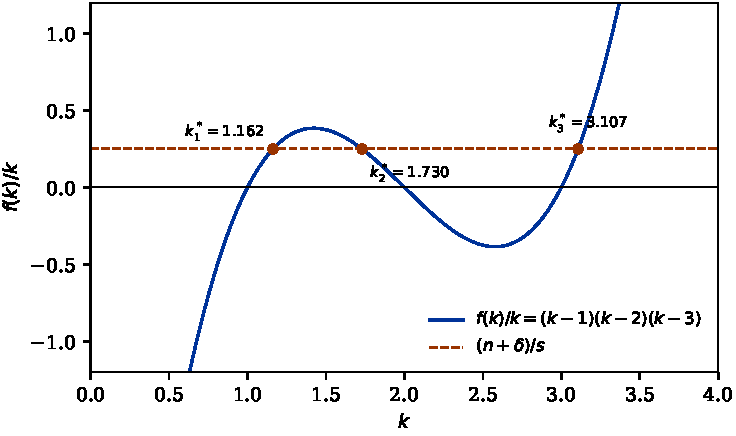
\includegraphics{figures/ch2_quartic_steady_states.pdf}
\caption{Steady states of the quartic economy: the interior steady states are the intersections of
$f(k)/k=(k-1)(k-2)(k-3)$ with the horizontal line $(n+\delta)/s$, drawn here at $1/4$.}
\label{fig:ch2quartic}
\end{figure}

\emph{(c) Stability.}  Since $\dt k=k\,s\bigl[(k-1)(k-2)(k-3)-h\bigr]$, the sign of $\dt k$ is the sign of
the vertical distance between the cubic and the line, and at a steady state
\[
\frac{\partial\dt k}{\partial k}\Big|_{k=k^*}=s\,k^*\cdot\frac{\dd}{\dd k}\Bigl[\frac{f(k)}{k}\Bigr]_{k=k^*},
\]
so a steady state is locally stable exactly when the cubic crosses the line \emph{downward}.  The cubic
crosses upward at $k^*_1$ (rising branch), downward at $k^*_2$ (falling branch), and upward again at
$k^*_3$:
\[
\text{at }k^*_1:\ +1.1045,\qquad
\text{at }k^*_2:\ -0.7820,\qquad
\text{at }k^*_3:\ +2.6774 ,
\]
for the derivative of $f(k)/k$.  Therefore $k^*_2$ is locally asymptotically stable while $k^*_1$ and
$k^*_3$ are unstable.  In addition $k=0$ is a rest point of the differential equation, and it is locally
stable: for small $k>0$ we have $f(k)/k<0<h$, so $\dt k<0$ and the economy collapses to zero.  The complete
phase line is
\[
\underbrace{0}_{\text{stable}}\ \longleftarrow\ \underbrace{k^*_1}_{\text{unstable}}\ \longrightarrow\
\underbrace{k^*_2}_{\text{stable}}\ \longleftarrow\ \underbrace{k^*_3}_{\text{unstable}}\ \longrightarrow\
\infty .
\]
An economy starting with $k(0)<k^*_1$ collapses to $k=0$; one starting in $(k^*_1,k^*_3)$ converges to
$k^*_2$; one starting above $k^*_3$ grows without bound.  This is a poverty-trap configuration: history
(the initial condition) decides the long-run outcome.

Finally, \emph{no} steady state can be globally stable.  Global asymptotic stability requires convergence
to the same point from every initial condition; but an economy that starts at another steady state stays
there forever, so the existence of more than one rest point rules global stability out immediately.

\rmk{Part (c) of the exercise asks one to prove that \emph{two} of the three steady states in (b) are
locally stable.  Of the three \emph{interior} steady states exactly one --- the middle one --- is locally
stable, as the sign pattern above shows: on the rising branches of $f(k)/k$ the economy is pushed away from
the steady state.  The count in the book is recovered only if the degenerate rest point $k=0$, which the
text elsewhere excludes as having ``no economic content'', is included among the steady states; then two of
the four rest points ($k=0$ and $k^*_2$) are stable and two are unstable.}
\end{aex}

\begin{aex}{2.5}{}
We must show that under \bk{Assumptions 1} and \bk{2} the continuous-time Solow model with population
growth at the rate $n$ has a unique steady-state equilibrium, with $k^*\in(0,\infty)$ solving \bk{(2.34)},
$y^*=f(k^*)$ and $c^*=(1-s)f(k^*)$.

By \bk{(2.33)} the equilibrium path satisfies $\dt k(t)/k(t)=sf(k(t))/k(t)-(n+\delta)$, so a steady state
with $k>0$ is precisely a solution of
\[
\psi(k)\equiv\frac{f(k)}{k}=\frac{n+\delta}{s} .
\tag{$*$}
\]

\emph{$\psi$ is continuous and strictly decreasing.}  Continuity is immediate from \bk{Assumption 1}.  For
monotonicity, differentiate:
\[
\psi'(k)=\frac{f'(k)k-f(k)}{k^2}=-\frac{w(k)}{k^2},
\qquad w(k)=f(k)-kf'(k) .
\]
Since $f$ is strictly concave with $f(0)=0$ (\bk{Assumption 2}), strict concavity gives
$f(k)>f(0)+kf'(k)=kf'(k)$, that is $w(k)>0$ for every $k>0$; equivalently, $w(k)=F_L>0$ is the wage, which
is positive by \bk{Assumption 1}.  Hence $\psi'(k)<0$ for all $k>0$.

\emph{The limits.}  Both $f(k)\to0$ and $k\to0$ as $k\to0$, so l'H\^opital's rule and \bk{Assumption 2}
give
\[
\lim_{k\to0}\psi(k)=\lim_{k\to0}f'(k)=\lim_{K\to0}F_K=\infty ,
\qquad
\lim_{k\to\infty}\psi(k)=\lim_{k\to\infty}f'(k)=\lim_{K\to\infty}F_K=0 .
\]
(The second limit also follows from $0<f(k)/k$ and concavity.)

\emph{Existence and uniqueness.}  $\psi$ is continuous on $(0,\infty)$ with limits $\infty$ at $0$ and $0$
at $\infty$, so by the Intermediate Value Theorem it attains the value $(n+\delta)/s>0$ at some
$k^*\in(0,\infty)$; since $\psi$ is strictly decreasing, that value is attained exactly once.  Hence there
is a unique steady-state capital-labor ratio, given by \bk{(2.34)}.

Finally, at $k^*$ the level of output per capita is $y^*=f(k^*)$ by definition of $f$, and since a constant
fraction $s$ of income is saved, consumption per capita is $c^*=(1-s)f(k^*)$, with the corresponding
investment $sf(k^*)=(n+\delta)k^*$ exactly replacing depreciated capital and equipping the new workers.

\rmk{The proof is that of \bk{Proposition 2.2} with $\delta$ replaced by $n+\delta$: going from discrete to
continuous time, and adding population growth, changes nothing essential.  Population growth acts exactly
like faster depreciation, since both erode the capital-labor ratio at a constant proportional rate.}
\end{aex}

\begin{aex}{2.6}{}
Let $f(k)=A\wt f(k)$ with $\wt f$ satisfying \bk{Assumptions 1} and \bk{2}, and let $k^*$ be the unique
steady state of Exercise 2.5, \ie the solution of
\[
G(k^*;A,s,\delta,n)\equiv sA\,\frac{\wt f(k^*)}{k^*}-(n+\delta)=0 .
\]
Writing $\wt w(k)\equiv\wt f(k)-k\wt f'(k)>0$ for the wage per unit of $A$, the computation in Exercise 2.5
gives
\[
\frac{\partial G}{\partial k^*}=sA\cdot\frac{\dd}{\dd k}\Bigl[\frac{\wt f(k)}{k}\Bigr]_{k=k^*}
=-\frac{sA\,\wt w(k^*)}{(k^*)^2}<0 ,
\]
so the Implicit Function Theorem applies at every parameter configuration and yields
$\partial k^*/\partial x=-(\partial G/\partial x)\big/(\partial G/\partial k^*)$ for each parameter $x$.
Since $\partial G/\partial A=s\wt f(k^*)/k^*>0$, $\partial G/\partial s=A\wt f(k^*)/k^*>0$,
$\partial G/\partial\delta=-1$ and $\partial G/\partial n=-1$,
\[
\frac{\partial k^*}{\partial A}=\frac{k^*\wt f(k^*)}{A\,\wt w(k^*)}>0,\qquad
\frac{\partial k^*}{\partial s}=\frac{k^*\wt f(k^*)}{s\,\wt w(k^*)}>0,\qquad
\frac{\partial k^*}{\partial\delta}=\frac{\partial k^*}{\partial n}
=-\frac{(k^*)^2}{sA\,\wt w(k^*)}<0 .
\]
This proves the four statements about $k^*$.

For output, $y^*=A\wt f(k^*)$, so for $x\in\{s,\delta,n\}$ the chain rule gives
\[
\frac{\partial y^*}{\partial x}=A\wt f'(k^*)\frac{\partial k^*}{\partial x},
\]
which has the same sign as $\partial k^*/\partial x$ because $\wt f'>0$: $\partial y^*/\partial s>0$ and
$\partial y^*/\partial\delta,\ \partial y^*/\partial n<0$.  For $A$ there is in addition a direct effect,
and both effects push the same way:
\[
\frac{\partial y^*}{\partial A}=\wt f(k^*)+A\wt f'(k^*)\frac{\partial k^*}{\partial A}>0 .
\]

The economics is transparent.  A higher saving rate or a better technology raises investment at every
capital-labor ratio and so shifts the $sf(k)/k$ schedule up, moving its intersection with the horizontal
line $n+\delta$ to the right.  A higher depreciation rate or a higher rate of population growth raises the
amount of investment needed merely to hold $k$ constant --- capital must be replaced, and new workers must
be equipped --- and so moves the intersection to the left.  The only new result relative to
\bk{Proposition 2.3} is the effect of $n$, and it enters exactly as $\delta$ does: countries with faster
population growth are, other things equal, poorer in per capita terms.
\end{aex}

\begin{aex}{2.8}{}
Throughout, $F$ is twice differentiable and exhibits constant returns to scale, $f(k)=F(k,1,A)$ is concave
(so $f''\le0$) with $f(0)=0$, and the Inada conditions of \bk{Assumption 2} hold.  What is \emph{not}
assumed is $F_{KK}<0$, $F_{LL}<0$, or even $F_K>0$ and $F_L>0$.  The first thing to notice is that the
missing sign restrictions on the first derivatives come for free.

\emph{Step 1: the marginal product of capital is nonnegative.}  Concavity makes $f'$ nonincreasing.  If
$f'(k_0)<0$ for some $k_0$, then $f'(k)\le f'(k_0)<0$ for every $k\ge k_0$, contradicting the Inada
condition $\lim_{k\to\infty}f'(k)=0$.  Hence $f'(k)\ge0$, that is $F_K\ge0$, for all $k>0$.  (One cannot
get more: a technology that is affine from some $k_0$ on has $f'\equiv0$ beyond $k_0$ and still satisfies
every hypothesis.  As the rest of the argument shows, $f'\ge0$ is all that is needed.)

\emph{Step 2: the wage is strictly positive.}  Write $w(k)=f(k)-kf'(k)$.  Since $f(0)=0$,
\[
w(k)=\int_0^k\bigl[f'(x)-f'(k)\bigr]\dd x ,
\]
and the integrand is nonnegative because $f'$ is nonincreasing.  It is moreover strictly positive on a set
of positive measure: $f'(x)\to\infty$ as $x\to0$ while $f'(k)<\infty$, so $f'(x)>f'(k)$ for all small $x$.
Hence $w(k)>0$ for every $k>0$; that is, $F_L>0$, and the ``not necessarily strictly'' concave technology
still pays a positive wage.

\emph{\bk{Proposition 2.2}: existence and uniqueness of the steady state.}  Exactly as in Exercise 2.5,
$\psi(k)\equiv f(k)/k$ satisfies $\psi'(k)=-w(k)/k^2<0$ by Step 2, so $\psi$ is \emph{strictly} decreasing
even though $f$ is only weakly concave.  Its limits are $\infty$ at $0$ and $0$ at $\infty$ by
\bk{Assumption 2} and l'H\^opital's rule.  The Intermediate Value Theorem therefore gives a unique
$k^*\in(0,\infty)$ with $f(k^*)/k^*=\delta/s$, and then $y^*=f(k^*)$ and $c^*=(1-s)f(k^*)$.  Nothing in the
argument used strict concavity; it used only that $w>0$, which Step 2 delivers.

\emph{\bk{Proposition 2.5}: global stability.}  Let $g(k)\equiv sf(k)+(1-\delta)k$, so that the discrete
time law of motion is $k(t+1)=g(k(t))$ and $k^*=g(k^*)$.  By Step 1, $g'(k)=sf'(k)+1-\delta>0$.  By Step 2,
$\delta=sf(k^*)/k^*>sf'(k^*)$, whence
\[
g'(k^*)=sf'(k^*)+1-\delta\in(0,1),
\]
and local stability follows from \bk{Corollary 2.1}.  For global stability, take $k(t)\in(0,k^*)$.  Since
$g$ is strictly increasing, $k(t+1)=g(k(t))<g(k^*)=k^*$; and since $\psi$ is strictly decreasing,
\[
\frac{k(t+1)-k(t)}{k(t)}=s\frac{f(k(t))}{k(t)}-\delta>s\frac{f(k^*)}{k^*}-\delta=0 .
\]
So $k(t+1)\in(k(t),k^*)$: the sequence is increasing and bounded above by $k^*$, hence convergent, and its
limit is a fixed point of $g$ in $(0,k^*]$, which can only be $k^*$ by uniqueness.  The argument starting
from $k(0)>k^*$ is identical with the inequalities reversed.  Monotone global convergence therefore
survives the weakening of \bk{Assumption 1}.

\emph{\bk{Proposition 2.6} must be weakened to weak monotonicity.}  The proposition asserts that
$\{w(t)\}$ is an increasing and $\{R(t)\}$ a decreasing sequence when $k(0)<k^*$.  With $f''\le0$ instead of
$f''<0$ we get
\[
R'(k)=f''(k)\le0
\qquad\text{and}\qquad
w'(k)=-kf''(k)\ge0 ,
\]
so the correct statement is that $\{w(t)\}$ is \emph{nondecreasing} and $\{R(t)\}$ is \emph{nonincreasing}
(with the inequalities reversed when $k(0)>k^*$).  Both can be locally constant: on any interval where $f$
is affine --- the production function is then locally an $AK$ technology --- the capital-labor ratio keeps
rising while factor prices do not move at all.  Strict monotonicity is restored as soon as $f''<0$ on the
relevant range, which is what \bk{Assumption 1} guarantees.
\end{aex}

\begin{aex}{2.9}{}
Let \bk{Assumptions 1} and \bk{2} hold and suppose $k(0)<k^*$.  By \bk{Proposition 2.5} the capital-labor
ratio increases monotonically to $k^*$: $k(t+1)>k(t)$ for every $t$, with $k(t)\to k^*$.

In equilibrium factor prices are the marginal products, and with constant returns they depend on the
capital-labor ratio alone:
\[
R(t)=F_K\bigl(K(t),L(t),A\bigr)=f'\bigl(k(t)\bigr),
\]
\[
w(t)=F_L\bigl(K(t),L(t),A\bigr)=f\bigl(k(t)\bigr)-k(t)f'\bigl(k(t)\bigr)=w\bigl(k(t)\bigr).
\]
Differentiating the two expressions in $k$,
\[
\frac{\dd R}{\dd k}=f''(k)<0,
\qquad
\frac{\dd w}{\dd k}=f'(k)-f'(k)-kf''(k)=-kf''(k)>0 ,
\]
both strict by \bk{Assumption 1}, which has $f''(k)=F_{KK}(k,1,A)<0$.

So $R(\cdot)$ is a strictly decreasing and $w(\cdot)$ a strictly increasing function of $k$.  Composing
with the strictly increasing sequence $\{k(t)\}$ gives
\[
w(t+1)=w\bigl(k(t+1)\bigr)>w\bigl(k(t)\bigr)=w(t),
\qquad
R(t+1)=f'\bigl(k(t+1)\bigr)<f'\bigl(k(t)\bigr)=R(t),
\]
that is, $\{w(t)\}_{t=0}^\infty$ is an increasing and $\{R(t)\}_{t=0}^\infty$ a decreasing sequence, and
they converge to $w(k^*)$ and $f'(k^*)$.  If instead $k(0)>k^*$, \bk{Proposition 2.5} gives a strictly
decreasing $\{k(t)\}$ and the two conclusions are reversed.

The economics is the usual scarcity argument: capital deepening makes capital abundant relative to labor,
so the marginal product of capital --- and with it the rental rate and the interest rate $r=R-\delta$ ---
falls, while the marginal product of labor, and hence the wage, rises.  Along the transition the entire
increase in output per worker that is not saved accrues to labor.
\end{aex}

\begin{aex}{2.10}{}
\emph{Part 1.}  The linear equation $\dt x(t)=ax(t)$ with $x(0)$ given has the unique solution
$x(t)=x(0)\exp(at)$.  If $a<0$ then $\exp(at)\to0$, so $x(t)\to0$ for every initial condition: the steady
state $x^*=0$ is globally asymptotically stable.  (If $a>0$ the solution diverges unless $x(0)=0$, and if
$a=0$ every point is a steady state.)

\emph{Part 2.}  Let $g$ be differentiable in a neighborhood of $x^*$, with $g(x^*)=0$ and $g'(x^*)<0$.  This
is the scalar case ($n=1$) of \bk{Theorem 2.5}: the Jacobian is the number $g'(x^*)$, its unique eigenvalue
is $g'(x^*)<0$, which has negative real part, so $x^*$ is locally asymptotically stable.  The direct
argument is just as short.  Since $g$ is continuous with $g(x^*)=0$ and $g'(x^*)<0$, there is
$\varepsilon>0$ with
\[
g(x)<0\ \text{ for }x\in(x^*,x^*+\varepsilon)
\qquad\text{and}\qquad
g(x)>0\ \text{ for }x\in(x^*-\varepsilon,x^*),
\]
so on that neighborhood $\dt x$ always points toward $x^*$; Part 3 applied to the interval
$(x^*-\varepsilon,x^*+\varepsilon)$ then gives convergence.

\emph{Part 3.}  Let $g$ be continuously differentiable with $g(x^*)=0$, $g(x)<0$ for $x>x^*$ and $g(x)>0$
for $x<x^*$.  Take any $x(0)<x^*$ (the case $x(0)>x^*$ is symmetric, and $x(0)=x^*$ is trivial).

Because $g$ is continuously differentiable it is locally Lipschitz, so by the Picard--Lindel\"of theorem
the solution through any point is unique.  The constant function $x\equiv x^*$ solves the equation, so the
trajectory starting below $x^*$ can never reach $x^*$ in finite time, and \emph{a fortiori} never crosses
it: $x(t)<x^*$ for all $t$.  Consequently $g(x(t))>0$ and $\dt x(t)>0$ for all $t$, so $x(\cdot)$ is
strictly increasing and bounded above by $x^*$.  A monotone bounded function converges; let
$L\equiv\lim_{t\to\infty}x(t)\le x^*$.

Suppose $L<x^*$.  By continuity $\dt x(t)=g(x(t))\to g(L)>0$, so there are $T$ and $\eta>0$ with
$\dt x(t)\ge\eta$ for all $t\ge T$, whence $x(t)\ge x(T)+\eta(t-T)\to\infty$, contradicting $x(t)\le x^*$.
Therefore $L=x^*$, and $x(t)\to x^*$ from every initial condition: $x^*$ is globally asymptotically stable.

\rmk{Part 3 is what makes the continuous-time Solow model so much better behaved than its discrete-time
counterpart.  In discrete time a one-dimensional map can jump over its fixed point, so a sign condition on
$g$ alone does not preclude two-cycles; \bk{Exercise 2.21} constructs exactly such a cycle.  In continuous
time trajectories are continuous and cannot cross a rest point, which is why the analogue of Part 3 fails
in discrete time.}
\end{aex}

\begin{aex}{2.13}{}
\emph{The law of motion.}  Labor income per worker is the wage $w(k)=f(k)-kf'(k)$, of which a fraction $s$
is saved; capital income $f'(k)k$ is entirely consumed.  Aggregate saving is therefore $sw(k(t))L(t)$, and
with population growth at the rate $n$ and depreciation $\delta$ the capital-labor ratio obeys
\[
\dt k(t)=s\,w\bigl(k(t)\bigr)-(n+\delta)k(t),
\qquad\text{so}\qquad
\frac{\dt k(t)}{k(t)}=s\,\phi\bigl(k(t)\bigr)-(n+\delta),
\qquad \phi(k)\equiv\frac{w(k)}{k}.
\]
Interior steady states are the solutions of
\[
\phi(k)=\frac{w(k)}{k}=\frac{n+\delta}{s} .
\tag{$*$}
\]
The contrast with the baseline model is exactly the replacement of $f(k)/k$ by $w(k)/k$.  In the baseline
model $f(k)/k$ is strictly decreasing, which is what delivered uniqueness in Exercise 2.5.  Nothing of the
sort holds for $w(k)/k$.

\emph{When is $\phi$ increasing?}  Differentiating,
\[
\phi'(k)=\frac{kw'(k)-w(k)}{k^2}
=\frac{-k^2f''(k)-w(k)}{k^2},
\]
using $w'(k)=-kf''(k)$.  Now recall that for a constant returns technology the elasticity of substitution
\bk{(2.37)} can be written as
\[
\sigma(k)=\frac{f'(k)\,w(k)}{-k\,f(k)\,f''(k)} ,
\]
so that $-k^2f''(k)=\alpha_K(k)\,w(k)/\sigma(k)$ with $\alpha_K(k)\equiv kf'(k)/f(k)$ the share of capital
in national income.  Substituting,
\[
\phi'(k)=\frac{w(k)}{k^2}\Bigl[\frac{\alpha_K(k)}{\sigma(k)}-1\Bigr],
\qquad\text{hence}\qquad
\phi'(k)>0\iff\sigma(k)<\alpha_K(k).
\]
So $w(k)/k$ rises precisely where capital and labor are hard to substitute relative to the capital share.
Intuitively, when $\sigma$ is small an increase in capital raises the wage more than proportionately,
because labor becomes the scarce complementary factor; saving out of wages then feeds back into more
capital, and the economy can have several rest points.

\emph{An explicit example.}  Let
\[
f(k)=A\bigl[\gamma k^{\rho}+(1-\gamma)\bigr]^{1/\rho}+Bk^{\alpha},
\qquad \rho=\frac{\sigma-1}{\sigma}<0,\quad\alpha\in(0,1),\ B>0 :
\]
a CES technology with a low elasticity of substitution plus a small Cobb--Douglas term.  Both terms are
increasing, strictly concave and homogeneous of degree one in $(K,L)$ when written as $Lf(K/L)$, so
\bk{Assumption 1} holds.  The CES term alone would violate \bk{Assumption 2}, since
$f'_{\text{CES}}(0)=A\gamma^{1/\rho}<\infty$ and $w_{\text{CES}}(\infty)=A(1-\gamma)^{1/\rho}<\infty$; the
Cobb--Douglas term repairs both, because $Bk^{\alpha}$ contributes $B\alpha k^{\alpha-1}\to\infty$ to
$f'(k)$ as $k\to0$ and $(1-\alpha)Bk^{\alpha}\to\infty$ to $w(k)$ as $k\to\infty$.  So $f$ satisfies
\bk{Assumptions 1} and \bk{2} in full, and
\[
w(k)=A(1-\gamma)\bigl[\gamma k^{\rho}+(1-\gamma)\bigr]^{(1-\rho)/\rho}+(1-\alpha)Bk^{\alpha} .
\]
Take $A=1$, $\gamma=1/2$, $\sigma=1/4$ (so $\rho=-3$), $B=0.02$ and $\alpha=1/2$.  Then $\phi(k)=w(k)/k$
falls from $+\infty$ to a local minimum $\phi=0.03005$ at $k=0.1509$, rises to a local maximum
$\phi=0.60360$ at $k=1.4340$, and falls back to $0$; the turning points are exactly where $\sigma(k)$
crosses $\alpha_K(k)$:
\[
\begin{array}{lcccc}
k & 0.05 & 0.30 & 1.00 & 3.00\\
\sigma(k) & 1.8871 & 0.3581 & 0.2537 & 0.3264\\
\alpha_K(k) & 0.9667 & 0.9603 & 0.5000 & 0.0483\\
\phi'(k) & -0.438 & +0.286 & +0.495 & -0.115
\end{array}
\]
Consequently ($*$) has \emph{three} solutions for every $(n+\delta)/s$ strictly between $0.03005$ and
$0.60360$.  With $(n+\delta)/s=0.045$ they are
\[
k^*_1=0.04972,\qquad k^*_2=0.27684,\qquad k^*_3=29.19752 ,
\]
and since $\dt k$ has the sign of $\phi(k)-(n+\delta)/s$, the outer two are locally asymptotically stable
($\phi'(k^*_1)=-0.442$, $\phi'(k^*_3)=-0.002$) while the middle one is unstable ($\phi'(k^*_2)=+0.240$).
Figure~\ref{fig:ch2wage} plots $\phi$ and the horizontal line.  The economy converges to the poor or to the
rich steady state according to whether it starts below or above $k^*_2$: with saving out of wages alone,
the Solow model produces a poverty trap.

\begin{figure}[htbp]
\centering
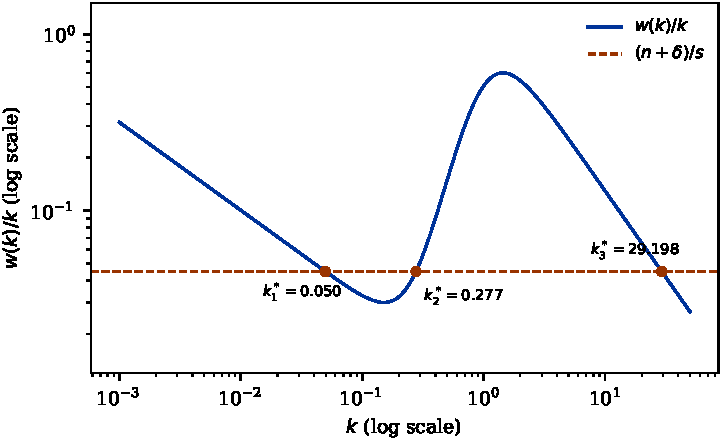
\includegraphics{figures/ch2_wage_savings_multiplicity.pdf}
\caption{Saving out of labor income only: steady states are the intersections of $w(k)/k$ with the
horizontal line $(n+\delta)/s$, drawn here at $0.045$, for the technology of the text.}
\label{fig:ch2wage}
\end{figure}

\rmk{The comparison with \bk{Exercise 2.12} is instructive.  When only capital income is saved, the law of
motion is $\dt k/k=s_Kf'(k)-(n+\delta)$, and $f'$ is strictly decreasing by \bk{Assumption 1}: the steady
state is unique and globally stable, whatever the elasticity of substitution.  It is the wage --- the
factor price that \emph{rises} with capital --- that can generate the self-reinforcing accumulation behind
multiplicity.}
\end{aex}

\begin{aex}{2.15}{}
With constant returns, output per worker and the wage are both functions of the capital-labor ratio alone:
\[
y=f(k),\qquad w=F_L=f(k)-kf'(k),
\]
the second equality being the competitive wage.  Along the family of economies indexed by $k$,
\[
\frac{\dd y}{\dd k}=f'(k),
\qquad
\frac{\dd w}{\dd k}=f'(k)-f'(k)-kf''(k)=-kf''(k)>0 ,
\]
so $w$ is a strictly increasing function of $k$ and can be inverted; by the chain rule,
\[
\frac{\partial y}{\partial w}=\frac{\dd y/\dd k}{\dd w/\dd k}=\frac{f'(k)}{-kf''(k)} .
\]
Therefore
\[
\varepsilon_{y,w}=\frac{\partial y}{\partial w}\cdot\frac{w}{y}
=\frac{f'(k)}{-kf''(k)}\cdot\frac{f(k)-kf'(k)}{f(k)}
=\frac{f'(k)\bigl[f(k)-kf'(k)\bigr]}{-k\,f(k)\,f''(k)} .
\tag{$*$}
\]

It remains to check that the right-hand side of ($*$) is the elasticity of substitution \bk{(2.37)}.  With
constant returns, $F_K=f'(k)$ and $F_L=f(k)-kf'(k)$, so
\[
\frac{\partial\log(F_K/F_L)}{\partial\log k}
=k\frac{\dd}{\dd k}\Bigl[\log f'(k)-\log\bigl(f(k)-kf'(k)\bigr)\Bigr]
=k\Bigl[\frac{f''(k)}{f'(k)}+\frac{kf''(k)}{f(k)-kf'(k)}\Bigr] .
\]
Putting the bracket over a common denominator,
\[
\frac{\partial\log(F_K/F_L)}{\partial\log k}
=k f''(k)\,\frac{\bigl[f(k)-kf'(k)\bigr]+kf'(k)}{f'(k)\bigl[f(k)-kf'(k)\bigr]}
=\frac{k\,f(k)\,f''(k)}{f'(k)\bigl[f(k)-kf'(k)\bigr]} ,
\]
and hence, by the definition \bk{(2.37)},
\[
\sigma=-\Bigl[\frac{\partial\log(F_K/F_L)}{\partial\log(K/L)}\Bigr]^{-1}
=\frac{f'(k)\bigl[f(k)-kf'(k)\bigr]}{-k\,f(k)\,f''(k)} ,
\]
which is exactly ($*$).  Therefore $\varepsilon_{y,w}=\sigma$.

The result is the basis of the empirical strategy of Arrow et al.\ (1961) taken up in
\bk{Exercise 2.16}: regressing the logarithm of output per capita on the logarithm of the wage across
economies (or across time) estimates the elasticity of substitution directly, and a slope of $1$ --- which
is what those authors found to be a good approximation --- says that the technology is Cobb--Douglas.  It
also gives a clean reading of $\sigma$: it measures how much richer, in output per worker, an economy must
be in order to sustain a given proportional increase in its wage.
\end{aex}

\begin{aex}{2.24}{}
Normalize the technology terms to $A_H=A_K=A_L=1$ (they only rescale the arguments and the level, and none
of the limits below depends on them) and write the per capita form of \bk{(2.38)} as
\[
f(k)=\bigl[\gamma k^{\rho}+(1-\gamma)\bigr]^{1/\rho},
\qquad \rho\equiv\frac{\sigma-1}{\sigma}\in(-\infty,1),\qquad\gamma\in(0,1),
\]
so that $\sigma>1\iff\rho\in(0,1)$, $\sigma<1\iff\rho<0$ and $\sigma=1$ is the Cobb--Douglas limit
$f(k)=k^{\gamma}$.  Differentiating,
\[
f'(k)=\gamma k^{\rho-1}\bigl[\gamma k^{\rho}+(1-\gamma)\bigr]^{(1-\rho)/\rho},
\qquad
w(k)=f(k)-kf'(k)=(1-\gamma)\bigl[\gamma k^{\rho}+(1-\gamma)\bigr]^{(1-\rho)/\rho} .
\]
Recall that \bk{Assumption 2} requires four limits --- $F_K\to\infty$ as $K\to0$, $F_K\to0$ as
$K\to\infty$, $F_L\to\infty$ as $L\to0$, $F_L\to0$ as $L\to\infty$ --- together with $F(0,L,A)=0$.  In per
capita terms $F_K=f'(k)$ and $F_L=w(k)$, and $L\to0$ with $K$ fixed means $k\to\infty$, while $L\to\infty$
means $k\to0$.

\emph{Case $\sigma>1$ (\ie $0<\rho<1$).}  As $k\to0$ the bracket tends to $1-\gamma>0$, so
\[
f(0)=(1-\gamma)^{1/\rho}>0 ,
\]
and capital is not essential: $F(0,L,A)>0$, the last requirement of \bk{Assumption 2}, fails.  As
$k\to\infty$ the bracket behaves like $\gamma k^{\rho}$, so
\[
f'(k)\longrightarrow\gamma k^{\rho-1}\bigl(\gamma k^{\rho}\bigr)^{(1-\rho)/\rho}
=\gamma^{1/\rho}>0 ,
\]
so $\lim_{K\to\infty}F_K=0$ fails too: the marginal product of capital is bounded below by a positive
number, and the technology is asymptotically linear in capital --- an $AK$ technology in the limit, which
is exactly why \bk{Exercise 2.23}(a) finds sustained growth in this case.  Finally, as $k\to0$ (that is,
$L\to\infty$ for given $K$), the bracket tends to $1-\gamma$ and
\[
w(k)\longrightarrow(1-\gamma)(1-\gamma)^{(1-\rho)/\rho}=(1-\gamma)^{1/\rho}>0 ,
\]
so $\lim_{L\to\infty}F_L=0$ fails as well: labor remains productive at the margin however abundant it is,
because output does not require capital.  (The two remaining limits, $f'(0)=\infty$ and
$w(\infty)=\infty$, do hold, the latter because $w(k)\sim(1-\gamma)\gamma^{(1-\rho)/\rho}k^{1-\rho}$
with $1-\rho>0$.)

\emph{Case $\sigma<1$ (\ie $\rho<0$).}  Now $k^{\rho}\to\infty$ as $k\to0$, so the bracket diverges and,
since $1/\rho<0$, $f(0)=0$: capital is essential, as \bk{Assumption 2} wants.  But
\[
f'(k)\longrightarrow\gamma k^{\rho-1}\bigl(\gamma k^{\rho}\bigr)^{(1-\rho)/\rho}=\gamma^{1/\rho}<\infty
\qquad\text{as }k\to0 ,
\]
so the Inada condition $\lim_{K\to0}F_K=\infty$ fails.  At the other end, as $k\to\infty$ the bracket tends
to $1-\gamma$ and
\[
w(k)\longrightarrow(1-\gamma)^{1/\rho}<\infty ,
\]
so $\lim_{L\to0}F_L=\infty$ fails as well.  (The two remaining limits, $f'(\infty)=0$ and $w(0)=0$, do
hold.)

\emph{Case $\sigma=1$.}  Then $f(k)=k^{\gamma}$ with $\gamma\in(0,1)$: $f(0)=0$,
$f'(k)=\gamma k^{\gamma-1}\to\infty$ as $k\to0$ and $\to0$ as $k\to\infty$, and
$w(k)=(1-\gamma)k^{\gamma}\to0$ as $k\to0$ and $\to\infty$ as $k\to\infty$.  All the requirements of
\bk{Assumption 2} hold.

Hence \bk{Assumption 2} holds for the CES technology if and only if $\sigma=1$.  The failure is
economically meaningful rather than technical: with $\sigma>1$ the two factors are good enough substitutes
that capital alone can produce, and accumulating it never drives its marginal product to zero; with
$\sigma<1$ they are such poor substitutes that the first units of capital are not infinitely productive,
and an economy with a fixed labor force cannot make the wage arbitrarily large.

\rmk{\bk{Assumption 1}, by contrast, holds for every finite $\sigma>0$.  Logarithmic differentiation of
$f'$ gives
\[
\frac{f''(k)}{f'(k)}=\frac{\rho-1}{k}+\frac{(1-\rho)\gamma k^{\rho-1}}{\gamma k^{\rho}+(1-\gamma)}
=-\frac{(1-\rho)(1-\gamma)}{k\bigl[\gamma k^{\rho}+(1-\gamma)\bigr]}<0
\qquad\text{for all }\rho<1 ,
\]
so $f''<0$, and $F_{KK},F_{LL}<0$ follow.  The text on page~55 states instead that ``the CES production
function with $\sigma>1$ violates Assumption 1''; what the computation above shows, and what this exercise
asks one to prove, is that what fails is \bk{Assumption 2}.}
\end{aex}

\begin{aex}{2.25}{}
With Harrod-neutral technological progress at the rate $g$ and population growth at the rate $n$, the
effective capital-labor ratio $k(t)=K(t)/\bigl(A(t)L(t)\bigr)$ obeys \bk{(2.51)}, and the BGP value $k^*$
solves \bk{(2.52)},
\[
H(k^*;s,\delta,n,g)\equiv s\,\frac{f(k^*)}{k^*}-(\delta+g+n)=0 .
\]

\emph{The level of technology does not enter.}  $A(0)$ appears nowhere in this equation --- it has been
normalized away by the definition of $k$ --- so
\[
\frac{\partial k^*\bigl(A(0),s,\delta,n,g\bigr)}{\partial A(0)}=0 .
\]

\emph{The other comparative statics.}  Exactly as in Exercise 2.5,
\[
\frac{\partial H}{\partial k^*}=s\cdot\frac{\dd}{\dd k}\Bigl[\frac{f(k)}{k}\Bigr]_{k=k^*}
=-\frac{s\,w(k^*)}{(k^*)^2}<0,
\]
where $w(k)=f(k)-kf'(k)>0$.  The Implicit Function Theorem applies and gives, with
$\partial H/\partial s=f(k^*)/k^*>0$ and $\partial H/\partial\delta=\partial H/\partial n=
\partial H/\partial g=-1$,
\[
\frac{\partial k^*}{\partial s}=\frac{k^*f(k^*)}{s\,w(k^*)}>0,
\qquad
\frac{\partial k^*}{\partial n}=\frac{\partial k^*}{\partial\delta}=\frac{\partial k^*}{\partial g}
=-\frac{(k^*)^2}{s\,w(k^*)}<0 .
\]

\emph{Output per capita.}  Along the BGP, income per capita is $y^*(t)=A(t)f(k^*)=A(0)e^{gt}f(k^*)$ by
\bk{(2.50)}.  Hence, for each $t$,
\[
\frac{\partial y^*}{\partial A(0)}=e^{gt}f(k^*)>0 ,
\]
which is the one comparative static that is new relative to \bk{Proposition 2.8}: a higher initial
technology level leaves the effective capital-labor ratio untouched but raises income per capita
proportionately, at every date.  For the remaining parameters the effect runs through $k^*$ alone,
\[
\frac{\partial y^*}{\partial x}=A(0)e^{gt}f'(k^*)\frac{\partial k^*}{\partial x},
\qquad x\in\{s,\delta,n\} ,
\]
which is positive for $s$ and negative for $\delta$ and $n$, since $f'>0$.

\rmk{The proposition lists no comparative static with respect to $g$, and for good reason: a higher $g$
lowers $k^*$ and hence the level of income per capita at any fixed date, but it raises its growth rate, so
$\partial y^*(t)/\partial g$ changes sign as $t$ grows.  This is the first appearance of a theme that
recurs throughout the book --- level effects and growth effects need not point the same way.}
\end{aex}

\begin{aex}{2.26}{}
Let \bk{Assumptions 1} and \bk{2} hold and consider the law of motion \bk{(2.51)} of the effective
capital-labor ratio,
\[
\dt k(t)=G\bigl(k(t)\bigr),
\qquad
G(k)\equiv sf(k)-(\delta+g+n)k .
\]
$G$ is continuously differentiable on $(0,\infty)$ by \bk{Assumption 1}, and by \bk{Proposition 2.11} it
has a unique zero $k^*\in(0,\infty)$, characterized by $f(k^*)/k^*=(\delta+g+n)/s$.

Write $G(k)=k\bigl[s\psi(k)-(\delta+g+n)\bigr]$ with $\psi(k)\equiv f(k)/k$.  As established in
Exercise 2.5, $\psi$ is strictly decreasing, with $\psi(k)\to\infty$ as $k\to0$ and $\psi(k)\to0$ as
$k\to\infty$.  Therefore
\[
k<k^*\implies\psi(k)>\psi(k^*)=\frac{\delta+g+n}{s}\implies G(k)>0 ,
\]
\[
k>k^*\implies\psi(k)<\psi(k^*)\implies G(k)<0 .
\]
That is exactly the hypothesis of part 3 of \bk{Corollary 2.2} (proved in Exercise 2.10), which therefore
gives global asymptotic stability: starting from any $k(0)>0$, $k(t)\to k^*$.  Moreover the convergence is
monotone, since $\dt k$ keeps a constant sign along the path: an economy that starts below its BGP
accumulates effective capital throughout the transition, and one that starts above decumulates it.

Local stability can also be read off the derivative at the rest point.  Using $sf(k^*)=(\delta+g+n)k^*$,
\[
G'(k^*)=sf'(k^*)-(\delta+g+n)=sf'(k^*)-\frac{sf(k^*)}{k^*}=-\frac{s\,w(k^*)}{k^*}<0 ,
\]
because the wage $w(k^*)=f(k^*)-k^*f'(k^*)$ is strictly positive.  So the linearization has a strictly
negative eigenvalue, confirming local asymptotic stability by part 2 of \bk{Corollary 2.2}, and giving in
addition the speed of convergence: near the BGP the gap $k(t)-k^*$ closes at the exponential rate
$s\,w(k^*)/k^*=(\delta+g+n)\,\alpha_L(k^*)$, where $\alpha_L=w/f$ is the share of labor in national income.

Since $k(t)\to k^*$ and $y(t)=A(t)f(k(t))$, output per capita converges to the balanced growth path
$A(0)e^{gt}f(k^*)$ and grows asymptotically at the rate $g$: with Harrod-neutral progress, transitional
dynamics and long-run growth separate cleanly, and the model behaves exactly as it did without
technological change once variables are measured per efficiency unit of labor.
\end{aex}

\end{document}
